\documentclass[12pt]{article}
 
\usepackage{multirow}
\usepackage{geometry}
\geometry{a4paper, margin=1in}
\usepackage{titlesec}
\usepackage{lipsum} % For placeholder text, remove this in your actual document
\usepackage{graphicx}
\usepackage{float}
\usepackage{amsmath}
\usepackage{titlesec}
\usepackage{hyperref}
\usepackage{enumitem}
\titleformat{\section}[block]{\filcenter\bfseries\Large}{\thesection.}{1em}{}


% Set the subsection title format
\titleformat{\subsection}
{\normalfont\large\bfseries}{\thesubsection}{1em}{}

\begin{document}

\title{HCI India Seminar Summary}
\author{Hariom Mewada\\
24M2137}
\maketitle

\newpage
\tableofcontents
\newpage

\section{November 7,2024}
% \subsection{To Do List}
% \begin{itemize}
%     \item Understand the Matchfixer system.
%     \item Setting up Matchfixer on local machine.
%     \item Understand How SSO Works.
%     \item Creating new branch to work on.
%     \item Feature to change TA vacancies for course

% \end{itemize}
\subsection{Summary of papers}
\subsubsection{Will Changing My Phone Make My
Photographs Better?}
\begin{enumerate}
    \item This study investigates whether there is a difference in perceived photograph quality between smartphones of different brands (iPhone and Android) and whether brand labels affect this perception.
    \item A within-subjects, counterbalanced study was conducted with 36 participants who assessed 36 photographs across three conditions: non-labelled, correctly labelled, and wrongly labelled.
    \item Results showed no significant difference in perceived photograph quality scores between iPhone and Android in the non-labelled condition ($p = 0.793$).
    \item However, the perceived quality scores significantly increased when a brand label was present (correct or wrong) ($p = 0.006$), indicating the influence of brand association on perceived value.
\end{enumerate}
\subsubsection{To Shuffle or Not to Shuffle: Evaluation of the
Effect of Shuffling on Celebrity Passfaces}
\begin{enumerate}
   
    \item This study examines the usability and memorability of Celebrity Passfaces under shuffled and non-shuffled grid conditions to address security concerns like shoulder-surfing and smudge attacks.
    \item A within-subjects, counterbalanced, longitudinal study with 100 university students compared performance across shuffled and non-shuffled grids.
    \item Results showed no significant difference in 10-day memorability between the conditions (shuffled: 98.97\%, non-shuffled: 96.91\%, $p = 0.3033$), indicating shuffling does not impair memorability.
    \item Recall time analysis highlighted differences in early vs. later recalls, but no significant differences were found overall, ensuring shuffled grids balance usability and security.
\end{enumerate}
\end{itemize}
    % \begin{enumerate}
    %     \item understood various modules of the intentor app like how
    %     \textbf  {dashboard}, \textbf{Challenges} and \textbf{Daily usage limit} works
    %     .
    %     \item Understood  \textbf{ Count of locks and usage count Notification}, \textbf{Login},\textbf{alertlaunch} subsection of the App.

         % \item Understand  \textbf{Frictional Challenges}, \textbf{Strict vs cancellabel},\textbf{Personal Stories} , \textbf{Sharing performace with friend} subsection of the library.
        
    %     \item Went through code  to understand their working. 
    % \end{enumerate}
    


\end{itemize}
    

%     \subsubsection{Meetings Key Decisions :} Decided to take demo from students who had worked on the library earlier ,take the access to the github repo,understand the functionality , report creation format and set timing for meeting with guide.

% \subsection{Understand How Session works}
%     \begin{enumerate}
%         \item \textbf{appActivityListener()} :
%         - It is a listener always present in the notification drawer. Whenever an
% app is launched or closed, the activity is noted and a callback is sent to the Restriction App.
%         \item understood various key functions implemented in the library \textbf{setSessionDuration}, \textbf{getSessionDuration}, \textbf{setInterSessionGap},\textbf{showRestrictionMessage},\textbf{startSessionTimer} etc.
%         \item when the app is launched session start time is recorded the we periodically fetch session start time and check difference with current time to check whethere the session is completed. once session ended intersession time is recorded and the same we do check intersession gap.
%         \item \textbf{Workflow:}
%             \begin{enumerate}
%                 \item appActivityListener() thread of RA starts listening from notification drawer.
%                 \item Open RA and navigate to the session interface to set session and intersession gap.
%                 \item \textbf{SetSessionDuration} and \textbf{SetInterSessionGap} from the library is called and data is saved.
%                 \item User Open Social Media App.
%                 \item From notification drawer callback is made to \textbf{appActivityListener() }.
%                 \item Call is made to \textbf{isWithinInterSessionGap} and if it returns true restriced message is shown else we start new session and user is permitted to used social media app untill the session ends.
%                 \item When \textbf{appActivityListener()} notes session time is finished it shows restricted message and callback is made to record intersession gap and \textbf{appActivityListener()} check the inter session gap . when the used tried to open the social media app during inter session gap it shows restricted message.
%                 \item once the social media app is closed a callback is made to library by appActivityListener()
%             \end{enumerate}
%     \end{enumerate}
%     \subsubsection{Meetings Key Decisions :}
%     \begin{enumerate}
%          \item Understand the working of library and explain the understanding with a ppt using the report and expain the working of varios modules of library;
%      \end{enumerate}

% \subsection{Adding the library as a dependency in the App} 
%     \begin{enumerate}
%         \item Include the library  in the settings.gradle file in main directory for creating build of the library along with app module and also include it in gradle.build of the app module to use it as a third party dependency.
%         % \begin{figure}[H]
%         % \centering
%         % 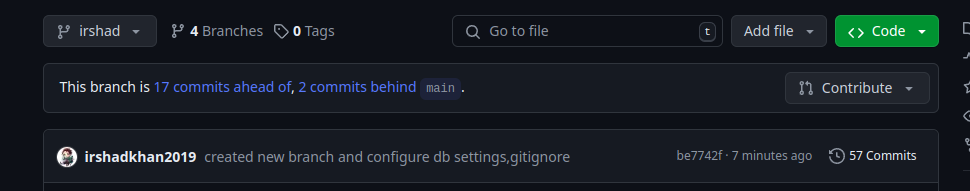
\includegraphics[width=15cm]{images/github.png}\\
%         % \caption{New branch creation}
%         % \label{fig: New branch created}
%         % \end{figure}
%     \end{enumerate}
% \section{August 12, 2024 - August 16, 2024}
% \subsection{Working of library}
%     \subsubsection{Importing various classes of library to use in Application}
%          \begin{enumerate}
%             \item Import \textbf{com.example.digitaldetoxkit.notificationlistener.NotificationListener},
%             \textbf{ com.example.digitaldetoxkit.pause.Pause} and 
%             \textbf{ com.example.digitaldetoxkit.analysis.analysis} classes in LoginActivity class of the application.
%         \end{enumerate}
%     % \subsection{Request Permission}
%     % \begin{enumerate}
%     %     \item Request the notificationn and overlay permission from user when first enter into the application.
%     % \end{enumerate}
%    \subsubsection{Setting up Analysis Service}
%          \begin{enumerate}
%             \item When the login activity is created , In the onCreate method of the Login Activity we start analysis service and it will keeps on running in background.
%             % \begin{figure}[H]
%             %     \centering
%             %     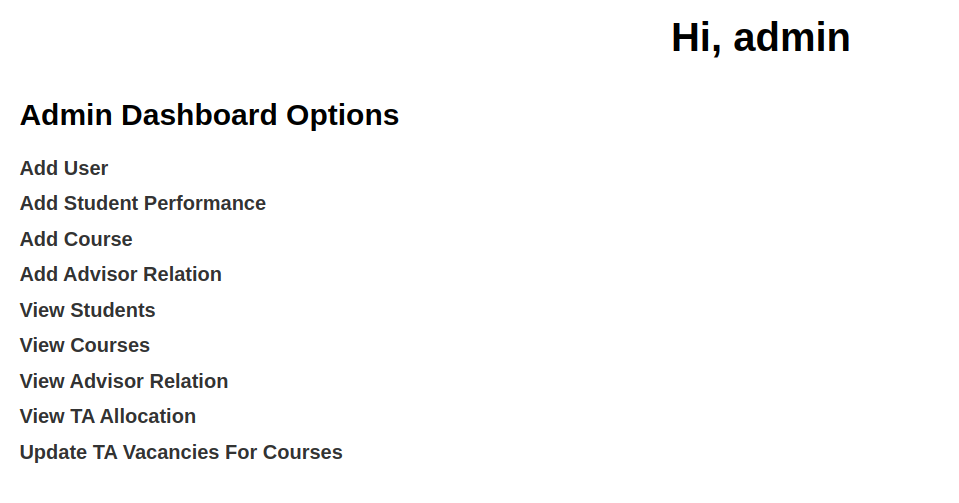
\includegraphics[width=18cm]{images/ta_vacancy_admin.png}\\
%             %     \caption{Update TA vacancies for courses}
%             %     \label{fig: Update TA vacancies for courses}
%             % \end{figure}
%             \item Create the Analysis class object by passing the activity name and application context in it's parameterized constructor.
%             \item Request the permission for usage statistics permission, if it's not granted already.
%          \end{enumerate}
% \subsection{Working of Analysis Service}
%           \subsubsection{Get Daily Screen Time}
%           \begin{enumerate}
%             \item \textbf{public List<Long> getDailyScreenTimeTrend(long startDate, long endDate)} method inside Analysis class is responsible to get daily screen time.
%             \item Inside \textbf{getDailyScreenTimeTrend} method we make query to system using \textbf{usageStatsManager} for getting resumed and stopped events between start and end date.
%             \item To calculate total duration of the app usage find the gap between stopped and resumed event for a particular package name .
%             \item  This method return list of Long in which every element represnt total usage time of the apps excluding system apps.
%             \end{enumerate}

%             \subsubsection{Get per App Usage for a Day}
%             \begin{enumerate}
%                 \item \textbf{Map<String, Long> getPerAppUsageForDay(long dateInMillis) }
%                 this method is responsible for calculating per app Usage for a day.
%                 \item This method accept  today's date in millisecond.
%                 \item working of the this same as \textbf{getDailyScreenTimeTrend} method the only difference is we return map of package name with the daily usage time to show app wise total usage time in day.
%             \end{enumerate}
%             \subsubsection{get Unlock Count}
%             \begin{enumerate}
%                 \item \textbf{public List<Long> getUnlockCount(long startdate, long enddate) } this method is responsible for getting unlcock count .
%                 \item \textbf{public Map<String, Long> getUnlockCountPerApp(long dateInmillis)} this method is repeated called from \textbf{getUnlockCount}.
                
%                 \item We have used \textbf{UsageStatsManager} to query an for the events in a particular duration and calpure all \textbf{MOVE TO FOREGROUND} events 
%                 \item for every \textbf{MOVE TO FOREGROUND}  we increament the count of   count for every app package and in the end we sum up all unlock counts to get total unlock count in the add.
                
%             \end{enumerate}
%     \subsection{Pausing the App}
%     \begin{enumerate}
%         \item Create \textbf{com.example.digitaldetoxkit.pause.Pause} class object in Login Activity of the application by passing activity and application context to it's constructor.
%         \item Ask for usage state permission and overlay permission from the user.
%         \item set pause duration for every package that we want to pause .
%         \item Start a thread that will periodically call \textbf{checkPackage} function to check if currently opened app is in the list of app to be paused.
%         \item once we detect the foreground app is in the list of apps that needs to be paused,we pause the app for given time interval and an overlay activity will be shown on the app for that time interval.
%     \end{enumerate}
%     \subsection{Notification Listner}
%     \begin{enumerate}
%         \item Create object of \textbf{com.example.digitaldetoxkit.notificationlistener.NotificationListener} class by passing activity name and application context;
%         \item Ask for the notification and notification listner permission using \textbf{notificationListener.SetPermissions()} method.
%         \item set notification schedule by calling \textbf{notificationListener.SetNotificationSchedule(time)} and pass the time interval for which we want to schedule the notification.
%         \item create the list of the apps for which we want to pause the notification 
%         \item call the method \textbf{notificationListener.BlockAppNotifications(appList)} for notification for apps present in appList.
%         \item This method will pass and intent to the \textbf{overrideNotification} service which contains information of the notification interval,blocked app list,allowed app list and application context will start \textbf{overrideNotification} service after this.
%         \item \textbf{onStartCommand} method will be called automatically once \textbf{overrideNotification}  service started.This method will call \textbf{BatchAndShowNotifications} for batch and show notifications.
%         \item Inside this function we will create a thread that will periodically check for the elapsedTime and once it is passed all the notifications are showed in batch.    
%     \end{enumerate}
%      \section{August 19, 2024 - August 23, 2024}   
     

% \begin{tabular}{ |p{4cm}|p{4cm}|p{4cm}|p {4cm} | }
%  \hline
%  \multicolumn{3}{|c|}{Feature List} \\
%  \hline
%  Feature Name & Implemented in library (Yes or No) &Implemented in App (Yes or No)  & Implemented Using Library(Yes or No)\\ 
%  \hline
%  Max Session Duration  & Yes   & Yes & No\\
%   \hline
%    InterSession Gap  & Yes   & No & No\\
%   \hline
% Scheduled Sessions&  Yes& No & No \\
%  \hline
% Daily Usage Limit & Yes & No & No\\
%  \hline
%  Batch Notifications  &Yes & No & No\\
%   \hline
%  Pause Before Usage&   Yes  & Yes & No\\
%   \hline
%  Analysis& Yes  & Yes   & No\\
%   \hline
%  Incentives& No  & No & No\\
%   \hline
%  Personal Stories& No  & No &  No\\
%   \hline
%  Friction Challenges& No  & Yes & No\\
%   \hline
% Strict vs Cancellable Restrictions& No  & No & No\\
%  \hline
% Sharing Performance with Friends& No  & No & No\\
%  \hline
% \end{tabular}


%  \section{August 26, 2024 - August 30, 2024} 
% \subsection{Max Session Duration And InterSession Gap API work flow and Code Snippets}
%  \begin{enumerate}
%      \item create object of \textbf{appActivityListener()} 
%  Service class inside the main activity of the RA and it will starts listening from the notification drawer.
%  \item From the session interface of RA set \textbf{Max Session Duration} and \textbf{Intersession Gap} for this \textbf{public boolean setSessionDuration(int durationInSeconds, String appPackageName)} and \textbf{ public boolean setInterSessionGap(int gapInSeconds, String appPackageName)} APIs are called from RA to library.
%  \item when the user opens the SM \textbf{appActivityListener()} will call \textbf{isWithinInterSessionGap(string appPackageName)}
%  to check if the SM is in the inner session gap,if it returns true then a callback is made from library to the app to show overlay popup that user is in the inter session gap and RA will launch the new activity which will appears on the SM app ,else if it return false usage is of SM app is permitted.
%  \item if the SM is not within the inter session gap then call is made to \textbf{startSessionTimer(string appPackageName, enum code)} it will starts the current session of the SM app.
%  \item when  \textbf{appActivityListener()}  noticed that session is finished by calling  \textbf{startSessionTimer(string appPackageName, enum code)} and pass enum code as \textbf{TIME FETCH }.it will made a callback to the RA and send the restriction message in the intent and RA will create new overlay activity  which will appear on the SM app with restriction message.
%  \end{enumerate}


%   \section{Sept 2, 2024 - Sept 13, 2024}
%   \subsection{Workflow Diagram of MaxSessionDuration and InterSessionGap}
%   \begin{enumerate}
%       \item
%   \begin{figure}[htp]
%     \centering
%     \includegraphics[width=18cm]{flawchar_session.png}
%     \caption{work flow diagram of session and inter session gap}
%     \label{fig:galaxy}
% \end{figure}
% +We have used \textbf{BroadcastReceiver} for communication between Library and RA.
% The \textbf{BroadcastReceiver} is a component in \textbf{Android} that listens for system-wide broadcast announcements or custom broadcasts. In our scenario, the \textbf{BroadcastReceiver} will listen for a broadcast from the \textbf{AppActivityListner} service with the result, and once the result is received, it will trigger the overlay activity.
% \end{enumerate}
% \subsection{Meeting Outcome}
% \begin{enumerate}
%     \item Start implemating the features from library on the intentor app latest code.
% \end{enumerate}

%  \section{Sept 15, 2024 - Sept 27, 2024}
%  \subsection{Environment SetUp}
%  \begin{enumerate}
%      \item Cloned Intentor from master branch.
%      \item created a new branch named digital detox hariom
%      \item Upgraded gradel and resolved some dependency version mismatch problem occured while creating build for existing code.
%      \item included library in root project and as a dependency for app module.
%      \item setup emulator for testing the app
%      \end{enumerate}
% \subsubsection{Implementation Of Creation Session Interface}
% \begin{enumerate}
% \item created a slider menu to display option for creating session.
% \item on clicking create max session duration option a new popup will occure for creating max session duration for  SM app.
% \item Now when user click on submit \textbf{setMaxSessionDuration} api of library is called from app and session duration and appName is passed through it .
% \item max session duration for the particular package name is saved and user is navigated to home page.
%  \end{enumerate}
%  \subsubsection{Meeting Outcome}
%  \begin{enumerate}
%      \item what happen when the session expire?implement the functionality of session expiry.
%  \end{enumerate}

%  \section{Sept 30, 2024 - oct 4, 2024}
%  \subsubsection{Storage of MaxSessionDuration info}
%  \begin{enumerate}
%      \item created table in squilite db for the session info.
%      \item table have following column - id,appName,MaxsessionDuration.
%      \item App Name have unique constraints
%      \item modified other classes  related to MaxSession duration to fit into current implementation .
%  \end{enumerate}
%  \subsubsection{Implementation Of Session Expiry}
%  \begin{enumerate}
%      \item  user open the SM app
%      \item session is started for the SM app
%      \item when the user continuously uses the app for MaxSession Duration then an overlay pop is shown on the SM app and current session info is deleted.
%      \item if the user closes the SM app before session Expiry then session info is deleted  and it will start new session when the user reopens the SM app.
%  \end{enumerate}

%  \section{oct 7,2024 - oct 13, 2024}
%   \subsubsection{Implementation Of Total usage time and total unlock count }
%   \begin{enumerate}
%       \item 
%   \end{enumerate}

%  \subsection{Workflow Diagram of Scheduled session}
%   \begin{enumerate}
%       \item
%   \begin{figure}[htp]
%     \centering
%     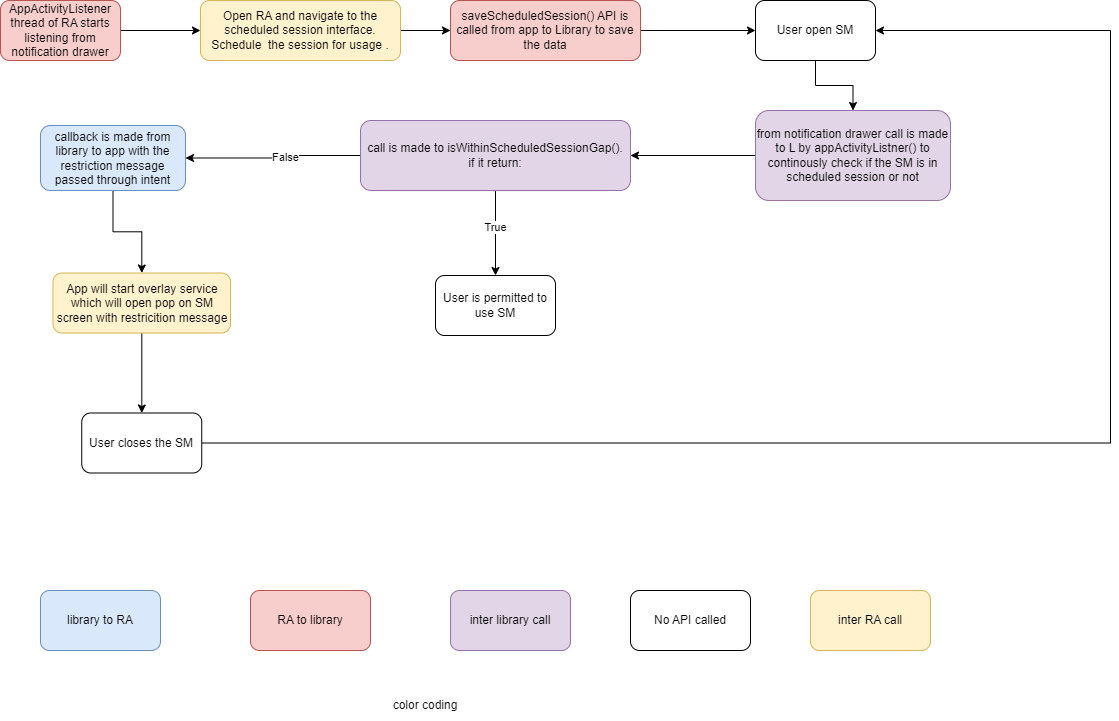
\includegraphics[width=18cm]{images/scheduled_session_implemented_drawio.png}
%     \caption{Workflow Diagram of Scheduled session}
%     \label{fig:galaxy}
% \end{figure}

% \subsection{Workflow Diagram of Daily usage limit and Max unlock count}
%   \begin{enumerate}
%       \item
%   \begin{figure}[htp]
%     \centering
%     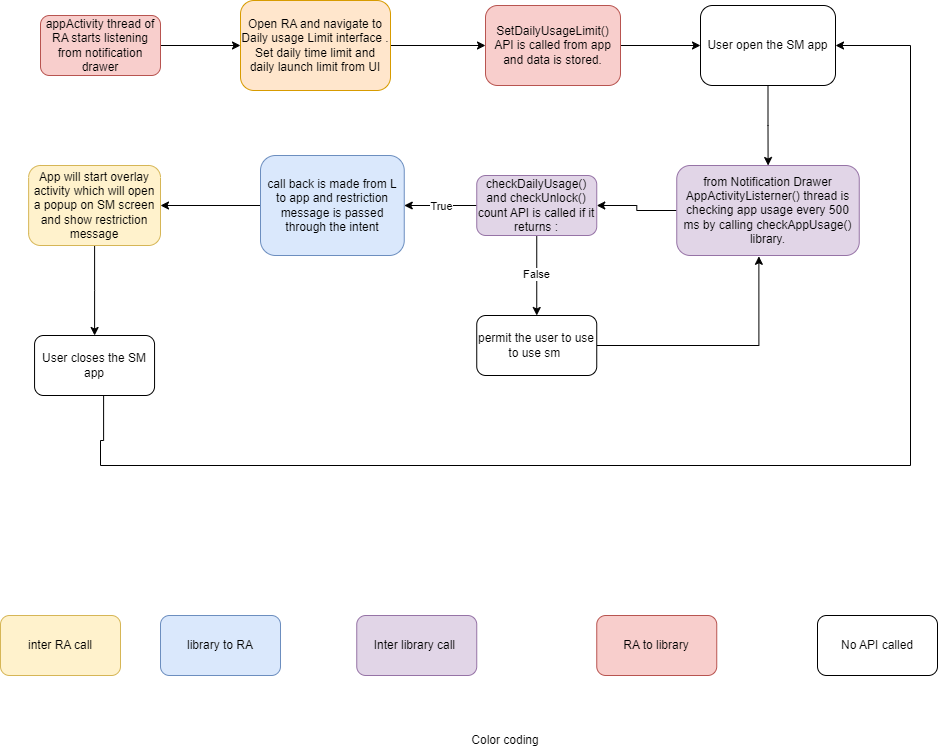
\includegraphics[width=18cm]{images/daily_usage_limit_drawio.png}
%     \caption{Workflow Diagram of Daily usage limit and Max unlock count}
%     \label{fig:galaxy}
% \end{figure}
    % \subsubsection{Workflow And Results}
    %     \begin{enumerate}
    %         \item On admin Dashboard ,user clicks Update TA vacancies for courses and is navigated to TA vacancies page which shows list of courses.
    %         \begin{figure}[H]
    %             \centering
    %             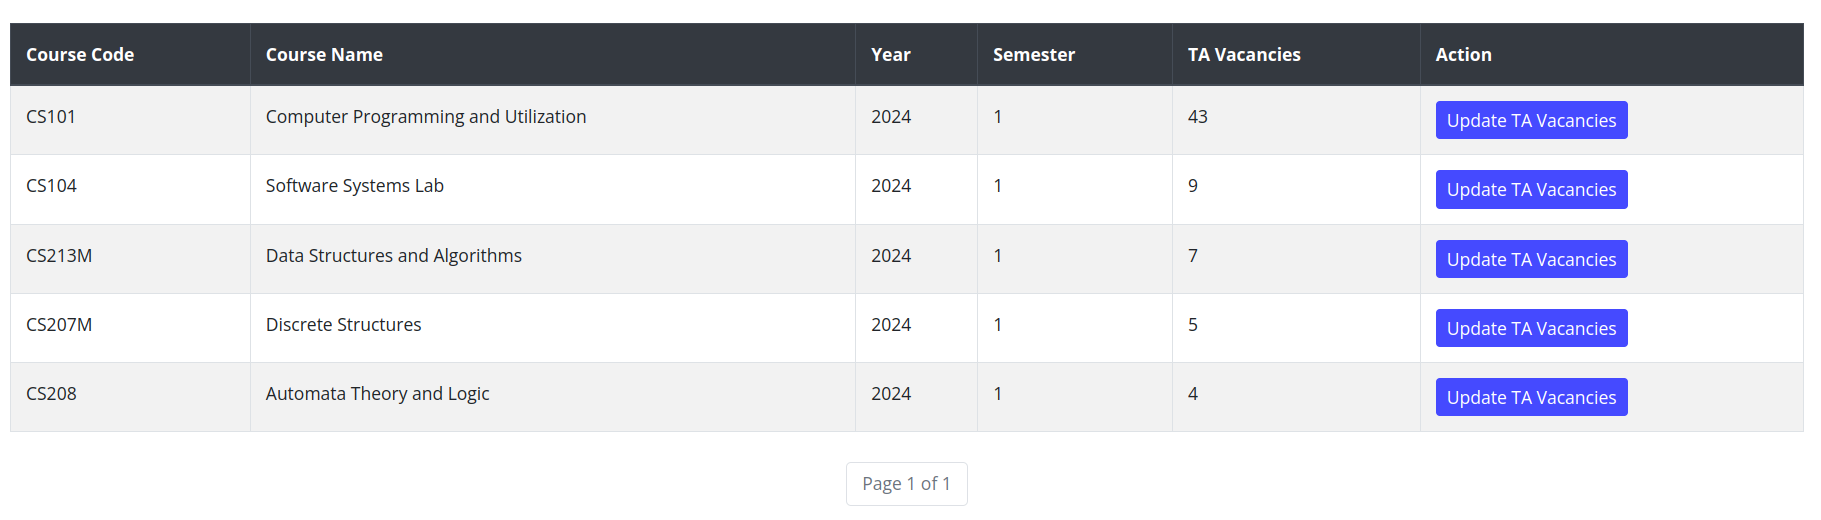
\includegraphics[width=18cm]{images/display_ta_vacancies.png}\\
    %             \caption{Display TA vacancies edit option}
    %             \label{fig: Display TA vacancies edit option}
    %         \end{figure}
    %         \item For a particular course when admin user clicks update TA vacancy,user is redirected to edit page.
    %         \begin{figure}[H]
    %             \centering
    %             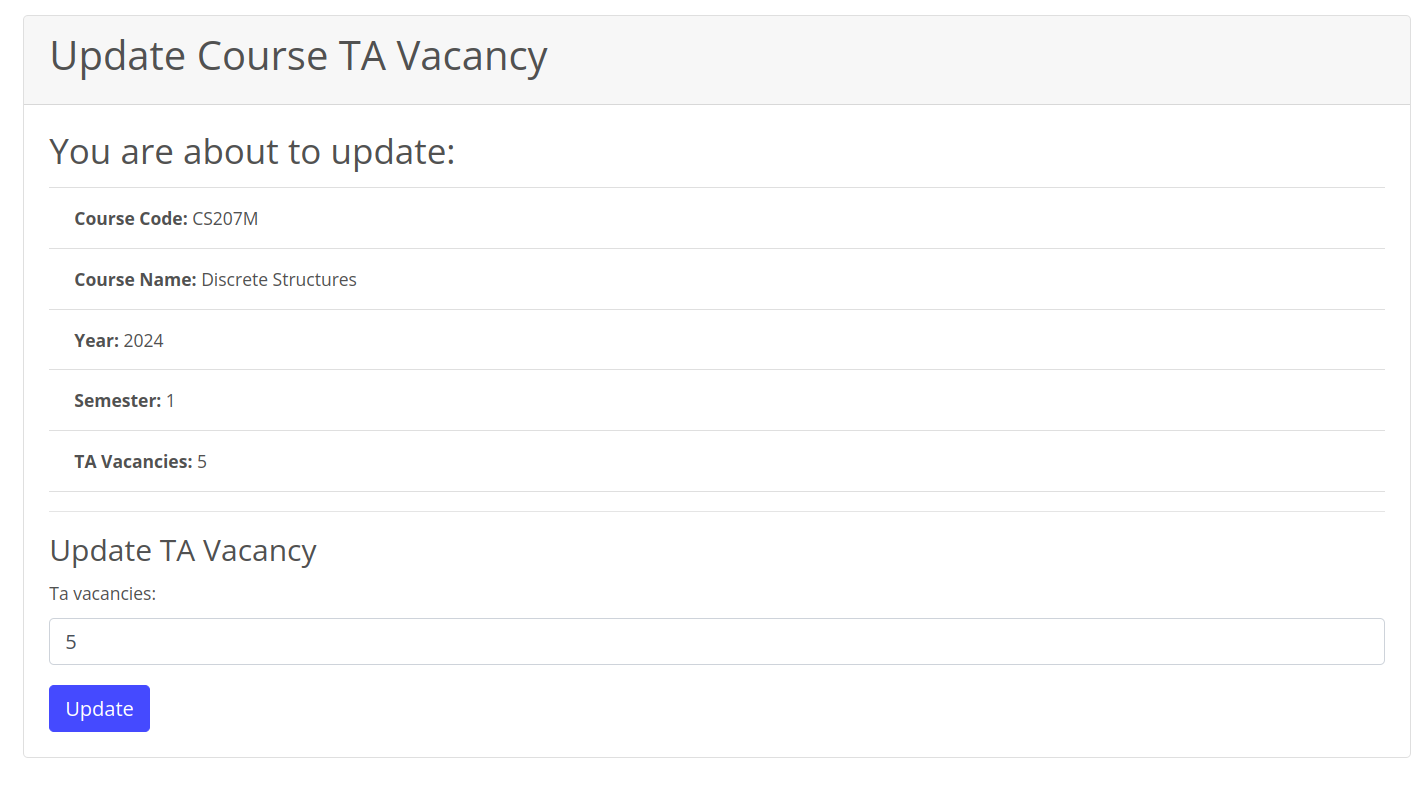
\includegraphics[width=18cm]{images/update_ta_vacancy.png}\\
    %             \caption{Display TA vacancies edit option}
    %             \label{fig: Display TA vacancies edit option}
    %         \end{figure}
    %         \item Select an appropriate value and click update.
    %         \begin{figure}[H]
    %         \centering
    %         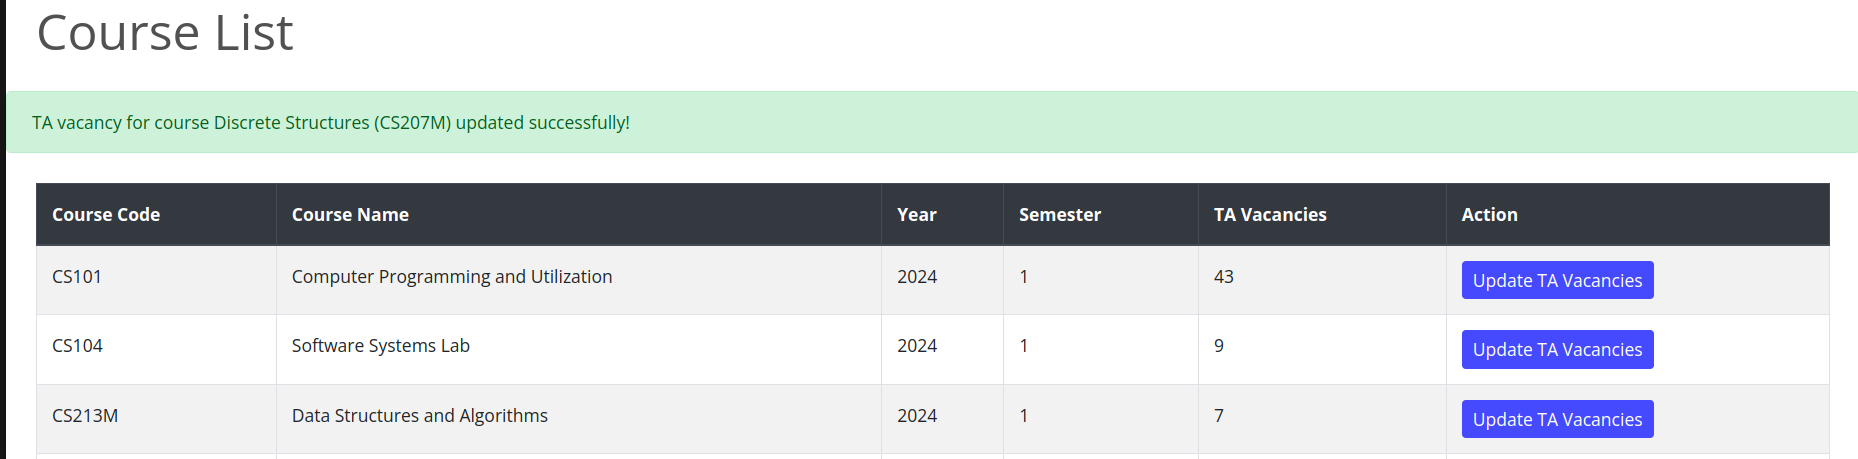
\includegraphics[width=18cm]{images/success_ta_vacancy.png}\\
    %         \caption{Successfully updated TA vacancy}
    %         \label{fig: Successfully updated TA vacancy}
    %         \end{figure}
    %         \item Done!
    %     \end{enumerate}
        
% \section{August 05, 2024 - August 11, 2024}
%     \subsection{Taking backup of prod code and db }
%       \begin{enumerate}
%           \item Backup of portal and DB running inside docker is stored in folder /home/matchfixer/backup.
%       \end{enumerate}
%     \subsection{Configuring SSL redirection }
%       \begin{enumerate}
%           \item \textbf{Production server} configured with nginx which servers as entrypoint to our server.
%           \item Matchfixer Container is now running on \textbf{port 8000} instead of 80 since port 80 is used by \textbf{nginx}.
%           \item Prod servers proxypass directive in NGINX is now used to forward client requests \textbf{from NGINX to matchfixer container} .
%           \item Configured nginx to \textbf{serve static and media files} from new/\texttt{Rnd\_portal} which is the \textbf{volume bind} for our matchfixer container.
%           \item Added \textbf{default login,logout and redirection url to /matchfixer} in settings.py and urls.py for our SSL redirection to work.(On github these changes not pushed yet.)
%           \item Matchfixer site made available at \textbf{matchfixer.cse.iitb.ac.in/matchfixer} for our https redirect to work from cse.iitb.ac.in/matchfixer. 
%           \item \textbf{Special thanks to Ranjith sir for guiding and configuring proxypass on cse.iitb.ac.in server}.
%       \end{enumerate}
      
%     \subsection{Design for Error checking on various CSV file input}
%      \subsubsection{Todo list}
%      \begin{enumerate}
%           \item Checking csv file reads for Authentication CsvUploader to upload users. Cores AdvisorUploader to upload Advisor.Cores CsvUploader to upload Courses,Cores GradeCsvUploader to upload Grades.
%           \item \textbf{Before storing} any data in db we need to make sure if all entries are valid .
%           \item Admin users must be notified at frontend which entries are not valid and they must rectify those entries to upload data .
%           \item Proper schema validation must be done if the csv follows correct schema as  db we must allow parsing of records.
%           % \ (***) If csv file data contains special characters like (,. etc) we need to store that also ??
%     \end{enumerate}
%     \subsubsection{ Design proposal}
%         \begin{enumerate}
%             \item When the csv file selected by admin user to upload ,first will \textbf{ check if it follows the correct schema} ,if not we can display that a particular field is missing please rectify it at front end upload csv views.
%             \item Eg. For student register we need \textbf{username,email,role,roll\_number,program,}\\\textbf{admission\_year} and if csv file doesn't has all these attributes can give schema validation error.
%             \item After schema validation we can loop through each records and check for any missing value and \textbf{push those records and errors in an array to display at front end} which record has issue and the respective error .
%             \item  If all validations pass,we can store entries in db.
%         \end{enumerate}
        
    
%     \subsection{Design for Admin interface to view/edit preference}
%         \subsubsection{Terminology}
%             \begin{enumerate}
%                 \item \textbf{StudentPreferences:} 
%                     \begin{enumerate}[label=\alph*.] % Change numbering to alphabetic
%                     \item Given by instructor .Here for a particular course and a particular student a preference value is given by instructor.
%                     \item A  course has \textbf{100*TaVacancies token} from which preference value is given.So Instructor can distribute total preference upto total course tokens.
%                     \item Eg.Total course \textbf{token= 500} then Instructor can use these 500 tokens as preference value and distribute to students
%                     \item Instructor can give\textbf{ max 120 }preference to a particular student.
%                 \end{enumerate}
            
%                 \item \textbf{CoursePreferences:} Given by Student.Here Student assign token to  a particular course. Student has \textbf{total 100 token} in total which he distributes to various courses.
%             \end{enumerate}
%          \subsubsection{Design for Admin interface to view/edit StudentPreferences}
%           \begin{enumerate}
%           \item \textbf{Suggestion 1:Meeting Discussion}
%           \begin{enumerate}[label=\alph*.] % Change numbering to alphabetic
%             \item Create a view for admins which shows all the StudentPref(course,student,prefernce value) and a \textbf{Download as csv btn} which downloads already stored preference in db as csv .
%             \item That view will also have \textbf{upload as csv} which after making changes to csv files admin can upload the changed preference value which will be stored in db.
%           \end{enumerate}
          
%           \item \textbf{Suggestion 2:} 
%                 \begin{enumerate}[label=\alph*.] % Change numbering to alphabetic
%                 \item Create a view which display \textbf{lists of students} which admin can select .
%                 \item For the \textbf{selected student} we can display all the StudentPreferences values assigned for different Course which will be \textbf{editable}.
%                 \item For the selected student,Can provide a \textbf{form to add new StudentPreferences}. 
%               \end{enumerate}
%           \end{enumerate}
%          \subsubsection{Design for Admin interface to view/edit CoursePreferences} 
%           \begin{enumerate}
%           \item \textbf{Suggestion 1:Meeting Discussion}
%           \begin{enumerate}[label=\alph*.] % Change numbering to alphabetic
%             \item Create a view for admins which shows all the CoursePref(course,student,token value) and a \textbf{Download as csv btn} which downloads already stored preference in db as csv .
%             \item That view will also have \textbf{upload as csv} which after making changes to csv files admin can upload the changed token value which will be stored in db.
%           \end{enumerate}
          
%           \item \textbf{Suggestion 2:} 
%                 \begin{enumerate}[label=\alph*.] % Change numbering to alphabetic
%                 \item Create a view which display \textbf{lists of students} which admin can select .
%                 \item For the \textbf{selected student} we can display all the CoursePreferences values assigned for different Course which will be \textbf{editable}.
%                 \item For the selected student,We Can provide an \textbf{form to add new CoursePreferences}.
%               \end{enumerate}
%           \end{enumerate}
%     \subsection{Design for Admin interface to view/edit advisor/student relation}
%     \subsubsection{View and Add advisor already availabe at admin interface} 
%             \begin{enumerate}[label=\alph*.] % Change numbering to alphabetic
%                 \item View advisor for a student is available at view\_advisors path .It displays mapping of Instructor to student.
%                 \item Add advisor for a student is available at advisor\_uploader path .It takes input as csv file with schema (instructorEmail,studentEmail) and stores each record in db.
%             \end{enumerate}
%      \subsubsection{Meeting Discussion}
%             \begin{enumerate}
%                 \item Instructor is advisor.
%                 \item A student can have one advisor(Instructor) and an Instructor can have many advisee(student). 
              
%             \end{enumerate}
%     \subsubsection{Design for Admin interface to edit advisor/student relation} 
%       \begin{enumerate}
%         \item \textbf{Suggestion 1:}
%         \begin{enumerate}[label=\alph*.] % Change numbering to alphabetic
%             \item Since we have a view which displays mapping of Instructor to student ,here itself we can provide edit btn which will take admin user to edit a relation view where admin can change a students advisor.
%             \item An Student have only one advisor,so we can provide a dropdown of all advisor which can be selected to change students current advisor.
        
            
%         \end{enumerate}
%         \item \textbf{Suggestion 2:}
%         \begin{enumerate}[label=\alph*.] % Change numbering to alphabetic
%             \item Since we have a view which displays mapping of Instructor to student ,here itself we can provide edit btn which will take admin user to edit a relation view where admin can change a Instructors advisees.
%             \item An Instructor can have many advisee ,so we need to display a list of already existing advisee for Instructor and an option to edit them .i.e remove/add new advisee for an Instructor.
            
%         \end{enumerate}
        
%      \end{enumerate}
    
 
\end{document}
